
We first notice that
\begin{equation}
    \pi_1(S^n)=\pi_1(\{*\}) = \{1\}
\end{equation}
for $n\geq 2$. But clearly $S^n$ is not homotopic to the one point
space $\{*\}$, i.e. $S^n$ is not contractible! Therefore, the
fundamental homotopy group does not solve the problem of determine the
homotopy of a space. The homology groups will be an new direction to go.

The details is covered in page 173 of \cite{book}.
Sadly, even if one can computes all the homology groups (or all the
homotopy groups), one cannot determine uniquely the homotopy type of
the space in general, unless one has some additional conditions.
For example, we have the Whitehead's Theorem: Given a continuous map
from $X\to Y$, two "good" topological spaces, if $f$ induces
isomorphisms on all homotopy group $\pi_n(X)\to\pi_n(Y)$, ($n\geq 1$),
and induces bijection on $\pi_0(X)\to\pi_0(Y)$, then $f$ is a
homotopic equivalence. Is there similar good theorem for homology
groups? Perhaps there is, but it is still not good enough for we still
need to find such a $f$.

Anyway, let's proceed to the discussion of simplicial homology.
\textbf{Note}: all the following discussions are based on a given
triangulation $K$ of the space.

\subsection{Section 8.1 - Cycles and boundaries}
\label{sec:Cycles-and-boundaries}

Geometrically, the homology groups aims to encode the information
about $k$-dimensional holes in a space, as holes are important in
determining the homotopy type of a space. 

Then we notice that the boundary and bulk relation is also important.
What I mean is in the following picture. The first loop encircles
a part that does not belong to the torus, whereas the second loop
encloses a solid part in the torus. One sees that the first loop is
not nullhomotopic, i.e. it cannot be homotopic contracted to the
trivial loop. On the other hand, loop 2 can. Look more generally, if a
loop is the boundary of simple part (e.g. a simplex), then it is
homotopic to the trivial loop. In this case we physicists can regard
it as the boundary of a good bulk, g simplex. However, if a loop has
empty bulk, i.e. it encloses no simplex, it is not a boundary of
something, then it will be a nontrivial element in the fundamental
group. This is why boundaries are important in our consideration.

\begin{figure}[H]
    \centering
    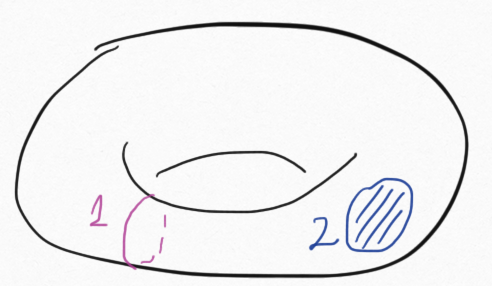
\includegraphics[width=0.6\linewidth]{pics/ch8/torus-p1.png}
\end{figure}

Before discussion, I should make clear that if we only care about
information of holes of certain dimension $q$, then we only have to care
about composition of simplexes of the same dimension $q$ that encloses
certain area (be it empty or not). For example, in fundamental groups,
we only care about holes looks like $S^1$. So in most cases we only
care about series of $1$-simplexes that is connected to form a loop,
as in the case of edge groups. We call these things that we care about
a closed $q$-cycles, to be defined precisely later.  The set of all
closed $q$-cycles are denoted $Z_q$.

Next is how to consider boundaries algebraically. For example, give a
set of vertices, how to seperate the boundary out of this? This is
especially troublesome given that we will have boundaries of different
dimensions. There are the $0$-dimension boundary of endpoints, the
$1$-dimension boundary of lines enclosing area, the $2$-dimension
boundaries called faces. 

The boundary operator $\partial$ aims to solve this problem, it gives
a systematic way to obtaining $(d-1)$-dimension boundary from a
$d$-dimension simplex. The simple examples are provided in page 174 to
175 of \cite{book}.

Lastly, as mentioned, closed $q$-cycles that is the boundary of some
solid part may become trivial, they are called $q$-boundaries. Closed
$q$-cycles that are not the boundary a solid part will be nontrivial.
Therefore, we might want to consider a quotient space:
$$ H_q = Z_q/B_q$$

I believe I have done a good job in summarizing the key point, now is
time to read the first section to get some practical ideas.

\subsection{Section 8.2 Homology groups}
\label{sec:Homology-groups}

This section formalize the intuitions from the previous section. It
defines \nomen{oriented simplex}, i.e. simplex denoted by a specific
$\{v_0,v_1,\vdots\}$ in this order. An change of order will change its
orientation. Such change of orientation is denoted by a minus sign,
and we have:
\begin{equation}
    (v_0,v_1,\cdots) = \operatorname{sign}\theta (v_{\theta(0)},
    v_{\theta(1)},\cdots)
\end{equation}
where $\theta$ is any permutation.

Then \nomen{$C_q(K)$} is the free abelian group generated by the oriented
$q$-simplexes of $K$, subject to the relations $\sigma+\tau=0$,
whenever $\sigma$ and $\tau$ are just the same simplex with opposite
orientations. An element of this group is called a \nomen{$q$-chain}.
Note that the rank of $C_q(K)$ is equal to the number of
$q$-simplexes in $K$.

The boundary homomorphism $\partial$ is defined such that
\begin{equation}
    \partial(v_0,\cdots,v_q)=\sum_{i=0}^{q}(-1)^i
    (v_{(0)},\cdots,\hat{v}_{(i)},\cdots,v_{(q)})
\end{equation}

where $(v_{(0)},\cdots,\hat{v}_{(i)},\cdots,v_{(q)})$
is shorthand for the oriented $(q-1)$-simplex obtained by deleting
the vertex $v_i$. It is easy to verify that $\partial^2=0$

In the special case when $q=0$, we define that boundary of a single
vertex is $0$ and that $C_{-1}(K)=0$.

We define the closed chains \nomen{$Z_q(K)$} as
\begin{equation}
    Z_q(K)=\Ker(\partial:C_q(K)\to C_{q-1}(K)).
\end{equation}
And the boundary \nomen{$B_q(K)$} is then
\begin{equation}
    B_q(K)=\Im(\partial:C_{q+1}(K)\to C_{q}(K)).
\end{equation}

$B_q$ will be a subgroup of $Z_q$ because $\partial^2=0$, this allows
us to define the \nomen{$q$-th homology group of $K$} as:
\begin{equation}
    H_q(K)=Z_q(K)/B_q(K)
\end{equation}

The elements of $H_q(K)$ are written $[z]$ for $z\in Z_q$, called the
\nomen{homology class} of $z$. Two $q$-cycles differ by a boundary
will have the same homology class and is called \nomen{homologous
cycles}. We note that $H_q(K)$ is by definition abelian and finitely
generated.

Of course, we need to verify various things in the above statements,
they can be found in the textbook \cite{book}.

\subsection{Section 8.3 Examples}
\label{sec:Section 8.3 Examples}

I will mention two theorems first:

\begin{thm}
    $H_0(K)$ is a free abelian group whose rank is the number of
    path-connected components of $|K|$ (or just components, as $|K|$
    is path-connected).
\end{thm}
\begin{proof}
    This is quite obvious.
\end{proof}

\begin{thm}
    If $|K|$ is connected, then $H_1(K)$ is isomorphic to the
    abelianization of its fundamental group $\pi_1(K)$.
\end{thm}
\begin{proof}
    Found on page 182 of \cite{book}.
\end{proof}

The two theorems indicates again that those homology groups are
independent of the choice of triangulation, and they should be
topological invariants. 

Then I will turn attention to specific examples.

\begin{key}
    \label{key:2cycle-orientation}
    Observe that every cycle is actually a closed object. It encircles
    or encloses an aresa. A closed $1$-cycle is actually a loop. A
    closed $2$-cycle will always enclose an area, so it is actually a
    sphere. A closed $2$-cycle will give an orientation on its
    surface. For example, suppose that we have a closed $2$-cycle
    $\lambda_i\sigma_i$, and assume that there is no repeated
    $2$-simple in this collection. For a given $2$-simplex $\sigma_1$
    in it, there will have to be $3$ simplexes surrounding it to
    cancal out $\sigma_1$'s edges. These $4$ $2$-simplexes are said to
    have compatible orientation. If one draw them on a paper, one will
    see that they are of the same orientation. Continue this argument
    to include all simplexes and one will see this $2$-cycle actually
    gives an orientation on its surface.
\end{key}
\begin{ex}\textbf{Torus}

    Consider the triangulation of torus as in
    exmaple~\ref{ex:triangu-torus}.
    \begin{figure}[H]
        \centering
        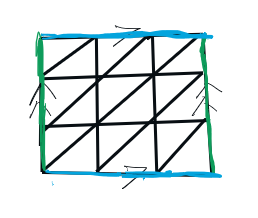
\includegraphics[width=0.6\linewidth]{pics/ch8/torus-tri.png}
    \end{figure}

    The zeroth homology group $H_0(K)$ marks the connected components,
    hence it is $H_0(K)=\Z$. The first homology group $H_1$ is about
    those closed loops. Almost all loops are boundaries. But there are
    two (the green one and the blue one), each of which cannot be a
    boundary. For example, I managed to make the orientation such that
    the green one is not cancelled, but this leaves a part of the blue
    one also un-cancelled. 
    \begin{figure}[H]
        \centering
        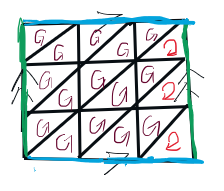
\includegraphics[width=0.6\linewidth]{pics/ch8/torus-tri-1.png}
    \end{figure}
    
    This two loops generates the $H_1(K)=\Z\cross\Z$, and are also the
    nontrivial objects in its fundamental group (a coindence,
    $\pi_1(T^2)=H_1(T^2)$).

    The $2$-cycles are easy to find. Because our space torus has no
    boundary, we have to add more and more $2$-simplexes until the
    whole space is covered with a $2$-chain. Then in this case, there
    is only one generator for $Z_2(K)$. Also, there is not
    $3$-simplex, so the $B_2=0$. Hence $H_2(K)=Z_2(K)=\Z$.
\end{ex}

\begin{ex} \textbf{Klein bottle $T^2$}

    As for the Klein bottle, I have had a hard time getting and
    confirming that the following is a triangulation:
    \footnote{
        I found two articles talking about minimal triangulations
        of Klein bottle. They are:
        \href{https://arxiv.org/abs/math/0407008}{link1}
        and
        \href{http://www.sciencedirect.com/science/article/pii/S0095895697999998}{link2}.
        The pdf files is also included.
    }
    \begin{figure}[H]
        \centering
        \includegraphics[width=0.6\linewidth]{pics/ch8/klein-tri.png}
    \end{figure}
    
    The $H_0(K)$ is clearly $\Z$.

    The $1$-cycles on this triangulation are hard to analyse. So I
    will use the fact that its $\pi_1=\braket{a,b|ba=a^{-1}b}$.
    The commutator is generated by $aba^{-1}b^{-1}=a^2$ and
    $bab^{-1}a^{-1}=a^{-2}$. So in the abelianization,
    $[a]=[a^{2n+1}]$, $[a^{2n}]=[1]$. So $[a]$ generates $\Z_2$. The
    $[b]$ is not affected, so $[b]$ generates $\Z$. It's easy to
    confirm that $[ab]=[ba]$, i.e. the abelianization group is
    abelian. All in all, $H_1(K)=\Z\cross\Z_2$.

    The $H_2(K)=0$, since there is no way to orient the Klein in a
    reasonable way (see key point~\ref{key:2cycle-orientation}).
\end{ex}

\begin{ex}\textbf{Cone Space}

    Now the book considers a complex $K$ which is a cone, i.e. $K$ is
    isomorphic to a complex of the form $CL$ where the dimentions of
    $L$ is $(\dim{K}-1)$.

    It is easy to see that $H_0(K)=\Z$, since cone is always
    connected.
    It is shown in page 181 of book\cite{book} that $H_n(K)=0$, for $n\geq
    1$. This is reasonable because cones are actually contractible, so
    there is not much interesting information about higher dimensional
    spheres in cones to be recorded. The book shows this by
    constructing a map $d:C_q(K)\to C_{q+1}(K)$, such that
    \begin{equation}
        \partial d(\sigma) = \sigma-d\partial(\sigma)
    \end{equation}
    It's easy to see that this means every closed cycle is a boundary.
\end{ex}

\begin{ex}\textbf{$(n+1)$-simplexes and $\sum^n\cong S^n$}

    Let $\Delta^{n+1}$ denotes a $(n+1)$-simplex. In this case, we
    consider it as a simplicial complex with all of its faces. Let
    $\sum^n$ denotes the simplexes which lies in the boundary of this
    $(n+1)$-simplex $\Delta^{n+1}$. Notice this is equivalent to say
    that $\sum^n$ is the all remaing simplex obtained by removing the
    interior points of $\Delta^{n+1}$. For example, $\sum^1$ is the
    3 edges and 3 vertices of the triangle. We see that $\sum^n$ is
    isomorphic to $S^n$.

    Every $\Delta^{n+1}$ can be thought of as a cone (except when
    $n=-1$, which is too trivial to be discussed here). So the
    homology classes of $\Delta^{n+1}$ are $H_0(\Delta^{n+1})=\Z$,
    $H_q(\Delta^{n+1})=0$, $q\geq 1$.
    
    The homology classes of $\sum^n$ can be calculated using
    $\Delta^{n+1}$, because they differ by only a single
    ${n+1}$-simplex, then most of their chains are the same.

    When $n=0$, the case is trivial and $H_0(\sum^0)=\Z\oplus\Z$,
    $H_q(\sum^0)=0$ for $q\geq 0$.

    When $n\geq 1$, then since $H_q$ does not involve simplexes of
    dimension higher than $q+1$, we have
    $H_q(\sum^n)=H_q(\Delta^{n+1})$, for $0\leq q\leq n-1$. Hence
    $H_0(\sum^n)=\Z$. $H_q(\sum^n)=0$, for $1\leq q \leq n-1$. 
    By using $H_n(\Delta^{n+1})=0$, it is easy to get
    $H_n(\sum^n)=\Z$. (book\cite{book} page 182). The rest of the Homology groups
    will of course be $0$.

    It is interesting to check that $H_n(\sum^n)=\Z$, not $0$ for a
    one point space. If we are able to show that Homology group is a
    topological invariant, then we know now Homology groups can be
    used to distinguish spheres with a point.
\end{ex}


\subsection{Section 8.4 Simplicial maps}
\label{sec:Simplicial maps}

Now we extend a simplicial map $K\to L$ to a homomorphism between
homology groups. This is easily done by first constructing
$s:C_q(K)\to C_q(L)$, and then confirming $s\partial=\partial s$, or
just $[s,\partial]=0$. This is a very general procedure and the
condition will be frequently seen in Homological algebra or
Cohomological algebra. In face, let me first introduces Homological
concepts first.

The collection of groups and homomorphisms:
$$\begin{tikzcd}[]
    \cdots \ar[r,"\partial"] & C_q(K) \ar[r,"\partial"] &
    C_{q-1}(K) \ar[r,"\partial"] & \cdots \ar[r,"\partial"] &
    C_0(K) \ar[r,"\partial"] & 0
\end{tikzcd}$$
will be called a \nomen{chain complex} of $K$, written $C(K)$. 
A \nomen{chain map} $\phi:C(K)\to C(L)$ is a set of group
homomorphisms $\phi:C_q(K)\to C_q(L)$. Such a map will induce a
homomorphism of Homology groups when $\phi\partial=\partial\phi$
(easily proved). This induced homomorphism between Homology groups is
dentoed $\phi_*$.

In our specific case where $s$ are simplicial maps $K\to L$, it is
easy to extend it to $s:C_q(K)\to C_q(L)$, since $s$ has already been
required to map simplexes to simplexes. We only need to pay attention
when $\sigma$ a generator (i.e. a $q$-simplex) of $C_q(K)$, is mapped
to a simplex of inferior quaility, i.e. of lower dimension $<q$. Then
it is nature to define $s(\sigma)=0$ in this case. It is verifed (page
185 of \cite{book}) that this map is well defined, is a homomorphism,
and has the property $s\partial=\partial s$. So $s$ induces a
homomorphism $s_*:H_q(K)\to H_q(L)$.
